\documentclass[margin=10pt]{standalone}    

\usepackage{tikz}
\usetikzlibrary{automata, positioning, arrows}

\begin{document}

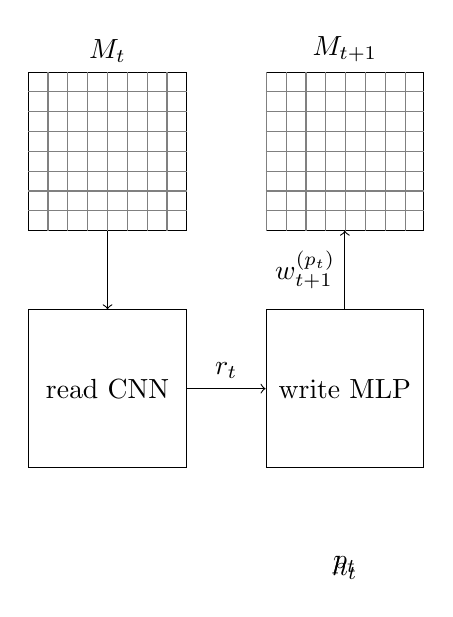
\begin{tikzpicture}[node distance=2cm]
    \tikzstyle{block} = [rectangle,minimum width=2cm,minimum height=2cm,text centered,draw=black,fill=white]

    \node (last) [block] {};
    \draw [step=0.252,gray,thin] (last.north west) grid (last.south east);
    \draw node [above=0cm of last] {$M_t$};

    \node (read) [block,below=1cm of last] {read CNN};
    \draw [->] (last) -- (read);

    \node (write) [block,right=1cm of read] {write MLP};
    \draw [->] (read) -- node [anchor=south]{$r_t$} (write);

    \node (next) [block,above=1cm of write] {};
    \draw [step=0.252,gray,thin] (next.north west) grid (next.south east);
    \draw node [above=0cm of next] {$M_{t+1}$};

    \draw [->] (write) -- node [anchor=east] {$w_{t+1}^{(p_t)}$} (next);

    \node (h) [below=1cm of write] {$h_t$};
    \node (p) [below=1cm of write] {$p_t$};

    %\draw [->] (h) -- (write);

    
    %\node (read) [block,above=1cm of write] {read CNN};
    %\draw [->] (read) -- (write);


\end{tikzpicture}

\end{document}
